%Preambulo---------------------------------------------------------------------------------------
\documentclass[11pt,a4paper]{article}
\usepackage[spanish]{babel}
\usepackage{graphicx}
\usepackage[margin=2.54cm]{geometry}
\usepackage[utf8]{inputenc}
\usepackage{ragged2e}
\usepackage[font = footnotesize,labelfont=it]{caption}
\usepackage{caption}
\usepackage{subcaption}


\pagestyle{empty}
%fin del preambulo-------------------------------------------------------------------------------

%Fin del preambulo-------------------------------------------------------------
\begin{document}
\begin{center}
{\textbf{\large Procesamiento de Señales Utilizando Herramientas Matemáticas y Computacionales para su Análisis\\}}
{\footnotesize Universidad Nacional Autónoma de México\\
Facultad de Estudios Superiores Cuautitlán\\} 
{\footnotesize Alonso Vargas Gachuz}
\end{center}

\begin{abstract}
La inteligencia artificial necesita tener acceso a una gran cantidad de información de la cual puede devolver una conclusión útil que podamos interpretar, en la mayoría de los casos la información obtenida no es apta para trabajarla, esta puede tener valores complejos o abstractos para el sistema imposibilitando la llegada a una conclusión. El preprocesamiento de la información es el primer paso para el desarrollo de sistemas inteligentes y quizá sea el más importante ya que aquí podemos encontrar y definir las características que nos interese averiguar. En este documento se relata el proceso para analizar y dar tratamiento de una base de datos la cual registra las vibraciones en los motores de ventilación con el fin de predecir una posible falla bajo diferentes condiciones. Se adecuaron los datos para su posterior uso en algún sistema. Para el procesamiento se proponen los siguientes pasos: limpiar y corregir datos faltantes, normalización, determinación de elementos estadísticos, determinación de cruces a cero, cambios de signo y aplicación de algoritmos para preprocesamiento. Con el fin de cumplir con estas tareas se usaron las herramientas Matlab y Python. Python fue usado para la limpieza y corrección de los datos mientras que Matlab se usó para el procesamiento de las señales y por su capacidad de realizar operaciones matemáticas. 
\end{abstract}

\section{Introducción}
El control, monitoreo y mantenimiento  de equipo para linea de producción son actividades fundamentales para la calidad y rendimiento de los procesos productivos. Los sensores y actuadores juegan un rol importante en la operación de varias maquinas como cintas transportadoras, generadores, mezcladoras, compresores, hornos, máquinas de soldar, entre otros, por lo que siempre deben operar en optimas condiciones, para garantizar esto, estas máquinas son constantemente monitoreadas \cite{accel_cite}
El diseño de cualquier sistema o dispositivo debe prever su uso y comportamiento en cualquier ambiente ya sea que existan condiciones inadecuadas o un mal manejo de estos. Un buen diseño debe contemplar estos aspectos y es por ello que se deben realizar pruebas en los dispositivos para conocer los limites de estos y prever el fallo en estos o advertir las condiciones en las que se deben operar. El proceso de prueba puede ser demasiado tardado si no se dispone de un antecedente o en caso de no saber por donde empezarlas. Para poder probar esta clase de motores se propone el uso de un sistema de predicción basado en un análisis previo, este sistema debe tener la capacidad de recolectar los datos y predecir el tiempo de falla de un motor según los parámetros de entrada. Como un primer paso para la creación de dicho sistema se debe emplear una base de datos de la cual dispongamos de la información necesaria para realizar el análisis adecuado. Con ayuda de una red neuronal es posible crear un sistema potente capaz de predecir la vida útil restante en motores, ya sea para prevenir fallas venideras e incluso para el análisis en el diseño de dispositivos que requieran el uso de motores con tal de hacer dispositivos más robustos que soporten mejor las vibraciones evitando daños importantes. Para este caso se usaron datos extraídos de una prueba con motores de ventilación, los parámetros medidos son: cambios de posición en los tres ejes (x,y,z) los cuales miden el desplazamiento del motor cuando se somete a vibraciones, configuración de peso: En la prueba se añadieron tres configuraciones de pesos en las aspas de los motores con el fin de producir las vibraciones en el motor que se busca medir(Figura 1), porcentaje de velocidad en revoluciones por minuto: porcentaje de velocidad en la que opera el motor.

\begin{figure}
	\centering
	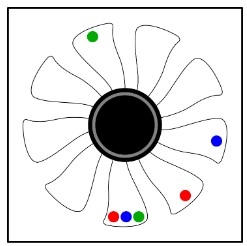
\includegraphics[scale=1]{weight_distr}
	\caption{Distribución de los pesos en las pruebas. 1.Rojo: Configuración normal. 2.Azul: Configuración perpendicular. 3.Verde: Configuración opuesta}
\end{figure}

\section{Conocimientos Previos}
\textbf{Transformada discreta de Fourier:} La transformada discreta de Fourier juega un rol clave en la física porque describe la relación entre el dominio del tiempo y el dominio de la frecuencia de señales discretas\cite{fourier}. Permite hacer un análisis de descomposición de cualquier tipo de señal y observar sus componentes con las cuales es posible realizar un análisis espectral en función de los resultados arrojados en el dominio de la frecuencia.

\textbf{Transformada Wavelet:} Las wavelets son señales, o formas de onda, las cuales tienen una duración limitada y un valor promedio de cero. Las wavelets pueden ser irregulares y asimétricas, características que les otorgan una mejor adaptación en el análisis de señales en comparación con la transformada de Fourier.\cite{intar}

\textbf{Análisis vibratorio}: La medición y análisis de vibraciones es utilizado, en conjunto con otras técnicas, en todo tipo de industrias como técnica de diagnostico de fallas y evaluación de la integridad de máquinas y estructuras. En el caso de los equipos rotatorios, la ventaja que representa el análisis respecto a otras técnicas como tintas penetrantes, radiografía, ultrasonido, etc., es que la evaluación se realiza con la máquina funcionando, evitando con ello la pérdida de producción que genera una detención\cite{analisis_vibr}.

\textbf{Procesamiento de Señales:} Se trata de una disciplina de las ciencias de la ingeniería que desarrolla las técnicas de procesamiento, análisis e interpretación. Entre las operaciones posibles con las señales tenemos control, filtrado, compresión de datos, deconvolución, predicción,etc.\cite{signal_processing}
\section{Metodología}
Con el fin de tratar los datos de las señales para que puedan ser interpretados por el sistema se deben realizar pasos de normalización y análisis de la información. Como primer paso se debe hacer una limpieza de los datos, normalización, búsqueda de información por medio de estadística descriptiva, búsqueda de picos y cruces a cero. A continuación se describe el método para el tratamiento de la base de datos. Dado que se empleó Matlab y Python con Jupyter los códigos del proceso descrito se encuentran en el siguiente repositorio de GitHub: \url{https://github.com/Kakoshi-ui/artificial\_intelligence\_2024\_I/tree/master/data\_processing\_act1/accelerometer}.
\subsection{Limpieza de datos}
Para verificar que no existan datos faltantes se utilizó el lenguaje de programación Python con la librería "Pandas" la cual nos permite trabajar con vectores y sus registros además de realizar cambios y búsquedas en la información. Con ayuda de la plataforma Jupyter y trabajando en Python podemos visualizar la información, es necesario añadirlas librerías de pandas, numpy y os para trabajar adecuadamente. Posteriormente se crea una instancia donde se guardará la base de datos empleada con el comando \textbf{pd.read.csv("Direction")} el cual importará los datos. una vez cargados verificamos datos faltantes con \textbf{datos\_completos.isnull()} el cual nos despliega una tabla en la que se verifica con sentencias lógicas si se poseen registros faltantes, también se puede usar el comando \textbf{.notnull()}. En caso de haber datos faltantes se usa el método \textbf{.dropna()} el cual filtra los registros que tengan valores NaN o nulos. Para completar los datos faltantes se puede usar el método \textbf{.bfill()} que permite rellenar los valores nulos con datos predefinidos. Para nuestro caso se verificó la posibilidad de encontrar datos faltantes, sin embargo la base se encuentra completa y no hubo necesidad de rellenar valores, aunque es importante siempre verificar la integridad de los datos en caso de usar archivos corruptos o por cualquier otra situación.

\subsection{Normalización de los datos}
A partir de este punto se usó unicamente la herramienta Matlab dada su buena capacidad para graficar y realizar operaciones matemáticas. Para normalizar los datos se calculan primero los valores máximos y mínimos de las funciones con los métodos \textbf{max(z)} y \textbf{min(z)} respectivamente. Posteriormente a la función original se le resta el valor mínimo para desplazar la función en caso que el valor resultante sea el mínimo y sea negativo. Al resultado de la operación se divide entre la suma del máximo y el mínimo, estableciendo así la normalización y resultando en valores entre cero y uno. La ecuación descrita es la siguiente: $zn = (z-minval(z))/(maxval(z)-minval(z))$

\subsection{Obtención de datos estadísticos}
En este punto se aplica la estadística descriptiva para obtener datos generales de la señal como es la media, mediana y moda de las señales. Para obtener estos valores se usan las funciones \textbf{mean(),median()} y \textbf{mode()} respectivamente.

\subsection{Cruces por cero ascendentes}
Una función continua puede presentar valores negativos y cambios abruptos de signo que son conocidos como cruces por cero, en nuestro caso estos representan el cambio de posición del motor con respecto a las vibraciones generadas lo cual es de interés. Para encontrar los cambios de signo se debe evaluar el producto del valor de la función en el punto i con el valor siguiente i+1 en caso que haya un cambio de signo significará que se encontró un cruce por cero, este método funciona de dos maneras: ubicando cruces ascendentes(cambios a signo positivo) o encontrando cruces descendentes(cambios a signo negativo). Por ello se evalúan los valores usando un ciclo y sentencias condicionadas.

\subsection{Preprocesamiento de señales}
Realizar un preprocesamiento a los datos nos puede arrojar aspectos interesantes de estas que no sean fáciles de encontrar en las señales originales, para ello se propone el análisis por medio de la Transformada de Fourier y la Transformada Wavelet. Para obtener las gráficas se usan los comandos \textbf{fft()} y \textbf{wavedec()}. Mientras que el método para obtener la transformada de fourier es simple, para obtener la transformada Wavelet se deben seguir algunos pasos extra:
\begin{enumerate}
	\item Se obtiene el vector de descomposición Wavelet y el número de coeficientes por nivel c y l respectivamente: $[c,l] = wavedec(x,n,wname)$. Dónde: 
	\begin{itemize}
		\item x es la función a la que se le aplica la transformada
		\item n es el nivel de descomposición de la transformada
		\item wname es la forma de la Wavelet madre que se va a emplear
	\end{itemize}
	\item Se obtienen los coeficientes de aproximación: $aprox = appcoef(c,l,wname)$
	\item Se obtienen los coeficientes de determinación, el vector de salida debe ser tan grande como el número de descomposición deseado: $d = detcoef(c,l,n)$. Dónde n es el número del nivel de descomposición.
\end{enumerate}

\section{Análisis de Resultados}

De los datos estadísticos pudimos recoger los siguientes valores de cada eje de movimiento
\begin{table}[h!]
	\centering

	\begin{tabular}{|c|c|c|c|c|c|}
	\hline
	Eje x & Valor & Eje Y & Valor & Eje Z & valor\\
	\hline
	Promedio & 0.9956 & Promedio & 0.0054 & Promedio & -0.1178\\
	\hline
	Mediana & 0.9920 & Mediana & 0.0080 & Mediana & -0.1250\\
	\hline
	Moda & 0.9800 & Moda & -0.0230 & Moda & -0.1210\\ \hline
	\end{tabular}
	\caption{Valores estadísticos de las señales}
	\label{table:1}
\end{table}
\\
Con los datos de la tabla podemos concluir que el eje x tiene una tendencia a desplazarse una unidad del lado positivo, mientras que el eje y permanece sin cambios significativos y se desplaza muy poco o casi nada. Por otro lado el eje z tiende a desplazarse ligeramente del lado de los valores negativos. De esto podemos concluir que en general es difícil que el motor se desplace a menos que se le someta a condiciones especificas.
\\
Antes de observar las gráficas es importante destacar los siguientes datos, donde se delimitan los valores de la configuración del peso y la velocidad angular del motor en dichos puntos para poder entender mejor los siguientes datos.
\begin{figure}[h!]
	\centering
	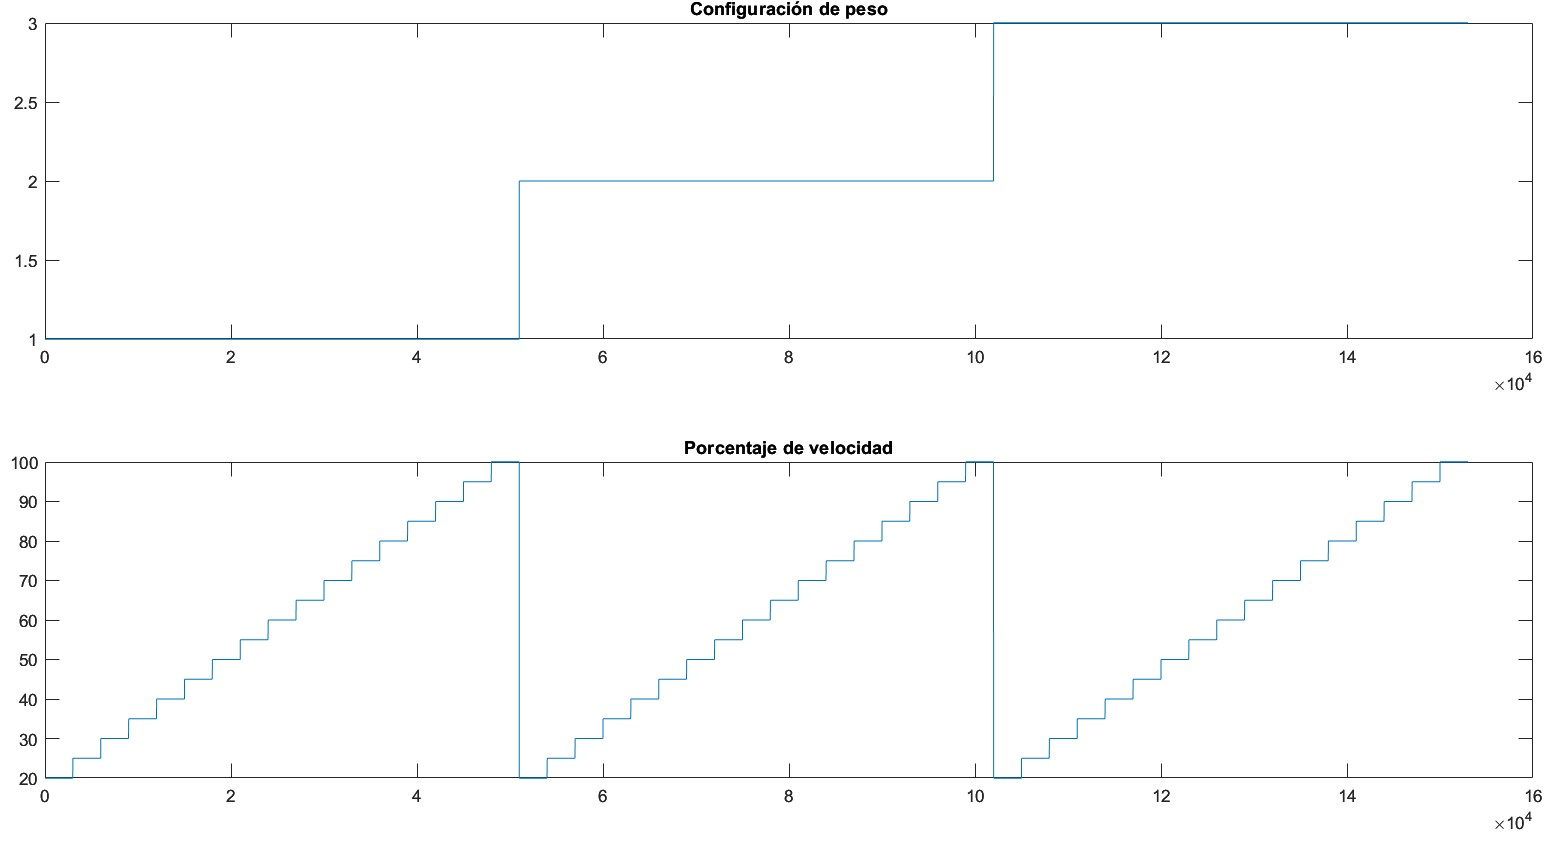
\includegraphics[scale=0.50]{w_rpm_conf}
	\caption{Grafica de arriba: Configuración del peso con 1=Rojo(configuración normal), 2=Azul(configuración perpendicular), 3=Verde(Configuración opuesta). Gráfica de abajo: porcentaje de RPM del motor}
\end{figure}
\\
Ahora observaremos los cambios de signo:
\\
\\
\\
\\
\begin{figure}[h!]
	\begin{subfigure}[b]{0.49\textwidth}
		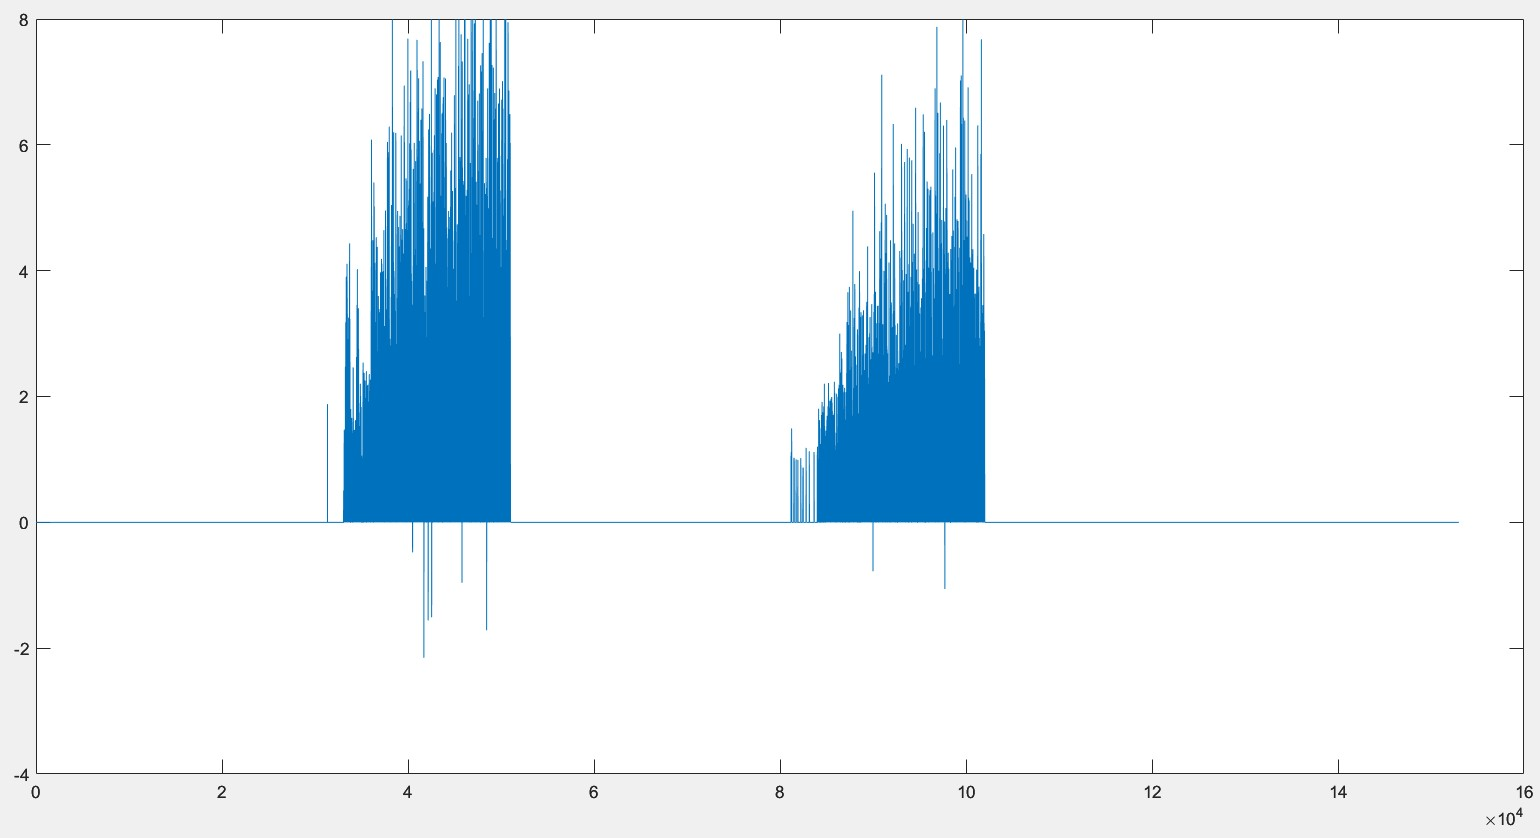
\includegraphics[scale=0.20]{zero_cross_x}
		\caption{Gráfica de cruces a cero en el eje X}
		\label{fig:f1}
		\hfill
	\end{subfigure}
	\begin{subfigure}[b]{0.49\textwidth}
		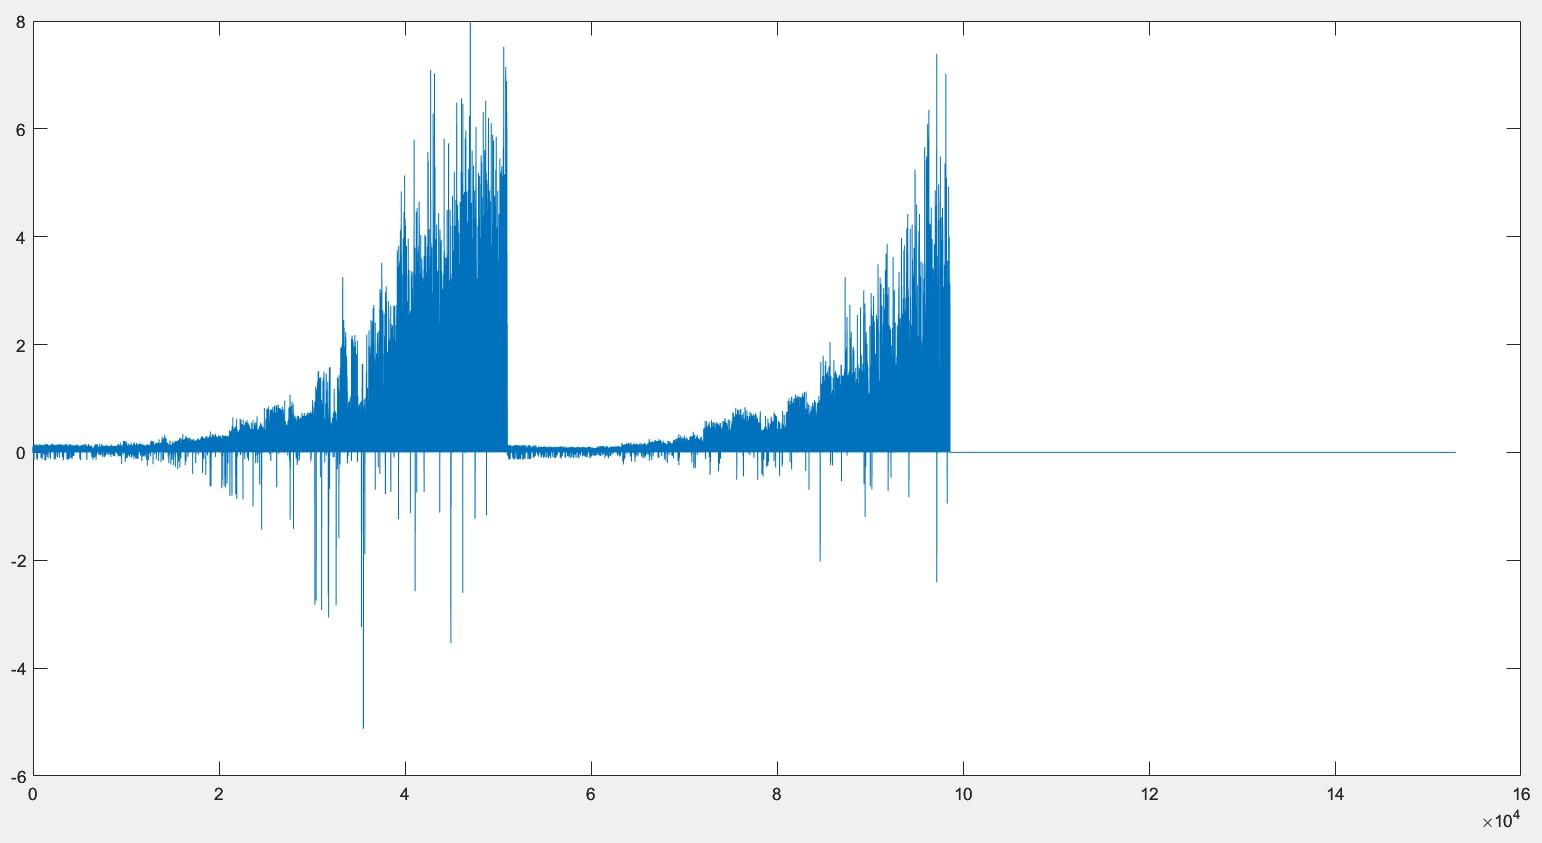
\includegraphics[scale=0.20]{zero_cross_y}
		\caption{Gráfica de cruces a cero en el eje Y}
		\label{fig:f2}
		\hfill
	\end{subfigure}
	\begin{subfigure}[b]{1\textwidth}
		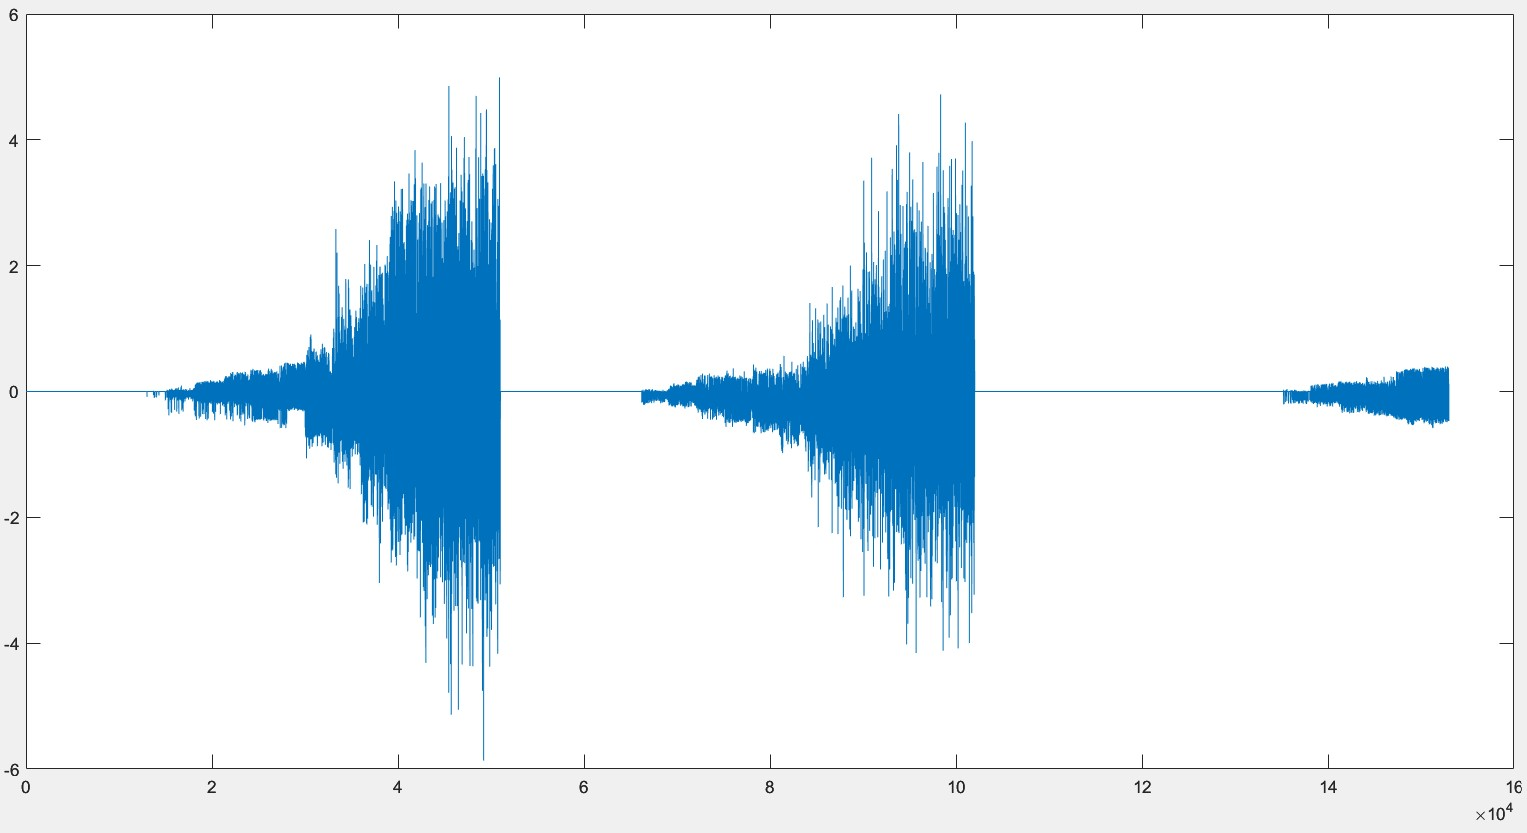
\includegraphics[scale=0.20]{zero_cross_z}
		\caption{Gráfica de cruces a cero en el eje Z}
		\label{fig:f3}
		\hfill
	\end{subfigure}
	\caption{Cruces a cero}
\end{figure}
Con las gráficas se puede observar que los principales cambios de signo se producen consecutivamente cuando el motor presenta muchas vibraciones y este aumento viene dado por el incremento en la velocidad angular del motor. Cuanto más se aumenten las revoluciones también incrementaran el número de vibraciones exceptuando por el caso de la configuración opuesta la cual es la que menos vibraciones tiene en general debido a la distribución del peso.
\\
Tras realizar un análisis podemos observar de mejor manera el comportamiento de las señales realizando un análisis espectral:
\begin{figure}[h!]
	\begin{subfigure}[b]{0.49\textwidth}
		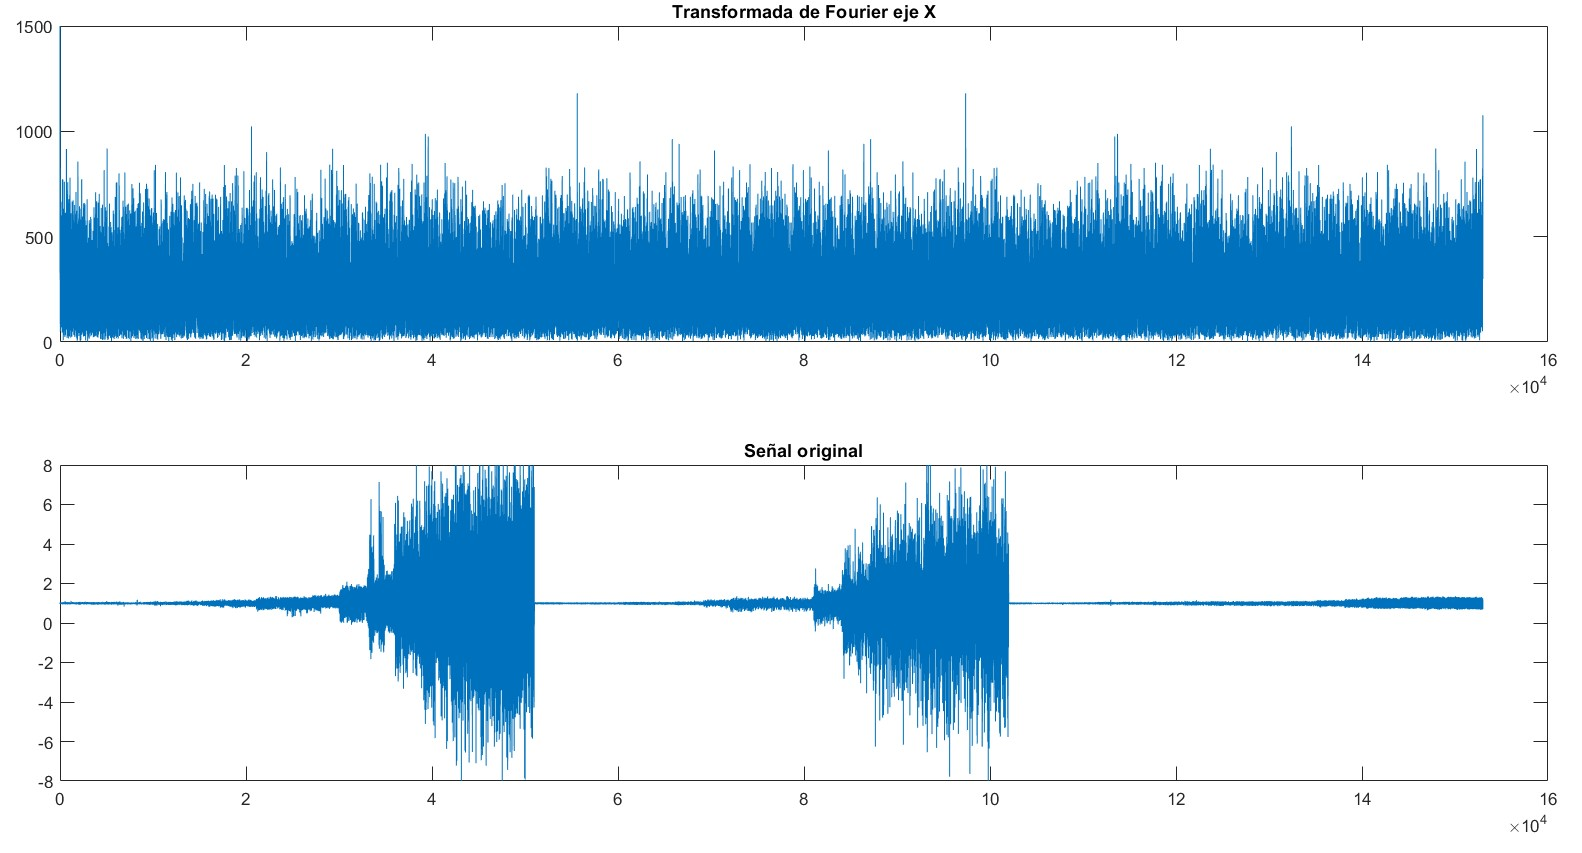
\includegraphics[scale=0.20]{fft_x}
		\caption{Análisis espectral en el eje X}
		\label{fig:f1}
		\hfill
	\end{subfigure}
	\begin{subfigure}[b]{0.49\textwidth}
		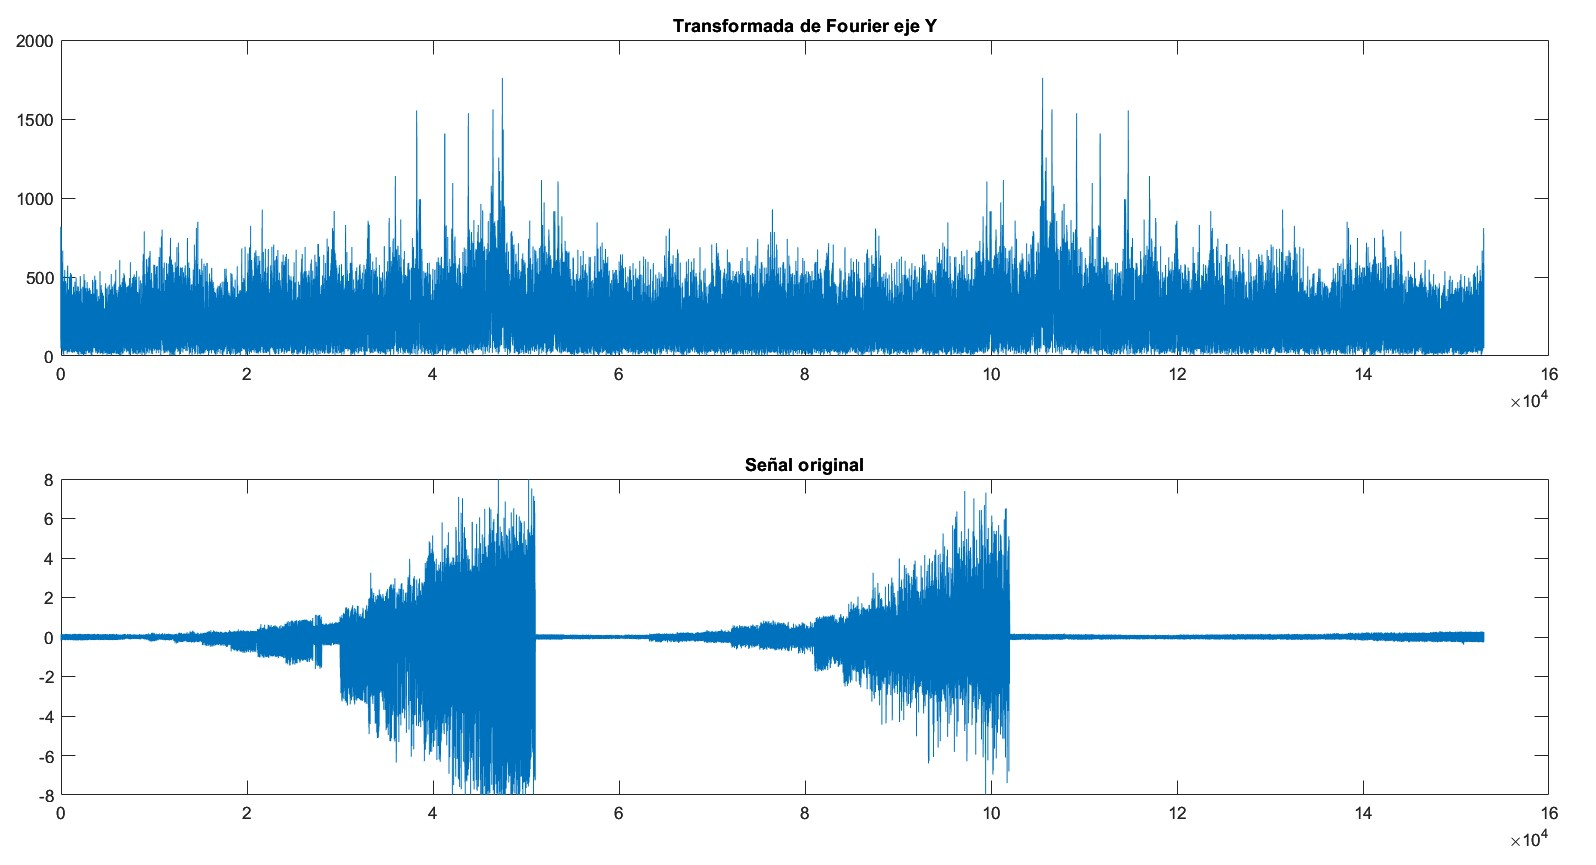
\includegraphics[scale=0.20]{fft_y}
		\caption{Análisis espectral en el eje Y}
		\label{fig:f2}
		\hfill
	\end{subfigure}
	\begin{subfigure}[b]{1\textwidth}
		\centering
		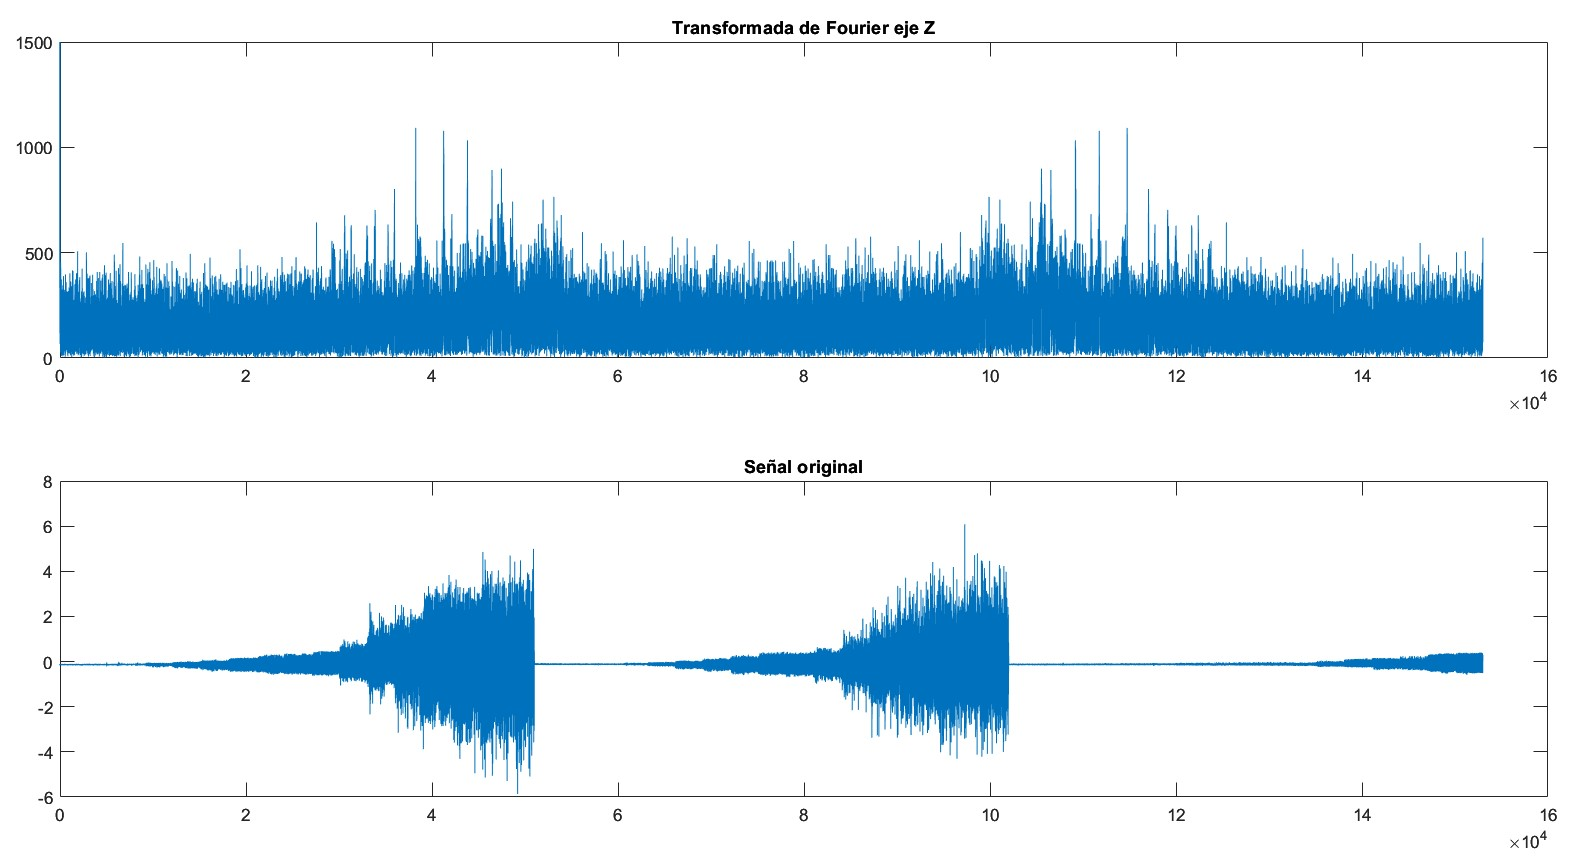
\includegraphics[scale=0.20]{fft_z}
		\caption{Análisis espectral en el eje Z}
		\label{fig:f3}
		\hfill
	\end{subfigure}
	\caption{Análisis de frecuencia en los tres ejes}
\end{figure}

Con ayuda de la gráfica en el dominio de la frecuencia podemos ver que el sistema es susceptible a cualquiera, sin embargo, es más sensible a determinadas frecuencias que son más visibles si se hace un análisis en profundidad. El problema al usar la transformada de Fourier es que el rango de frecuencias es muy grande y se vuelve complicado observar las aspectos más importantes del comportamiento de la señal. Para observar con más detenimiento es que se usa la transformada Wavelet que entrega mejor resolución de las señales en altas frecuencias.
\\
Análisis con transformada Wavelet:
\begin{figure}[h!]
	\centering
	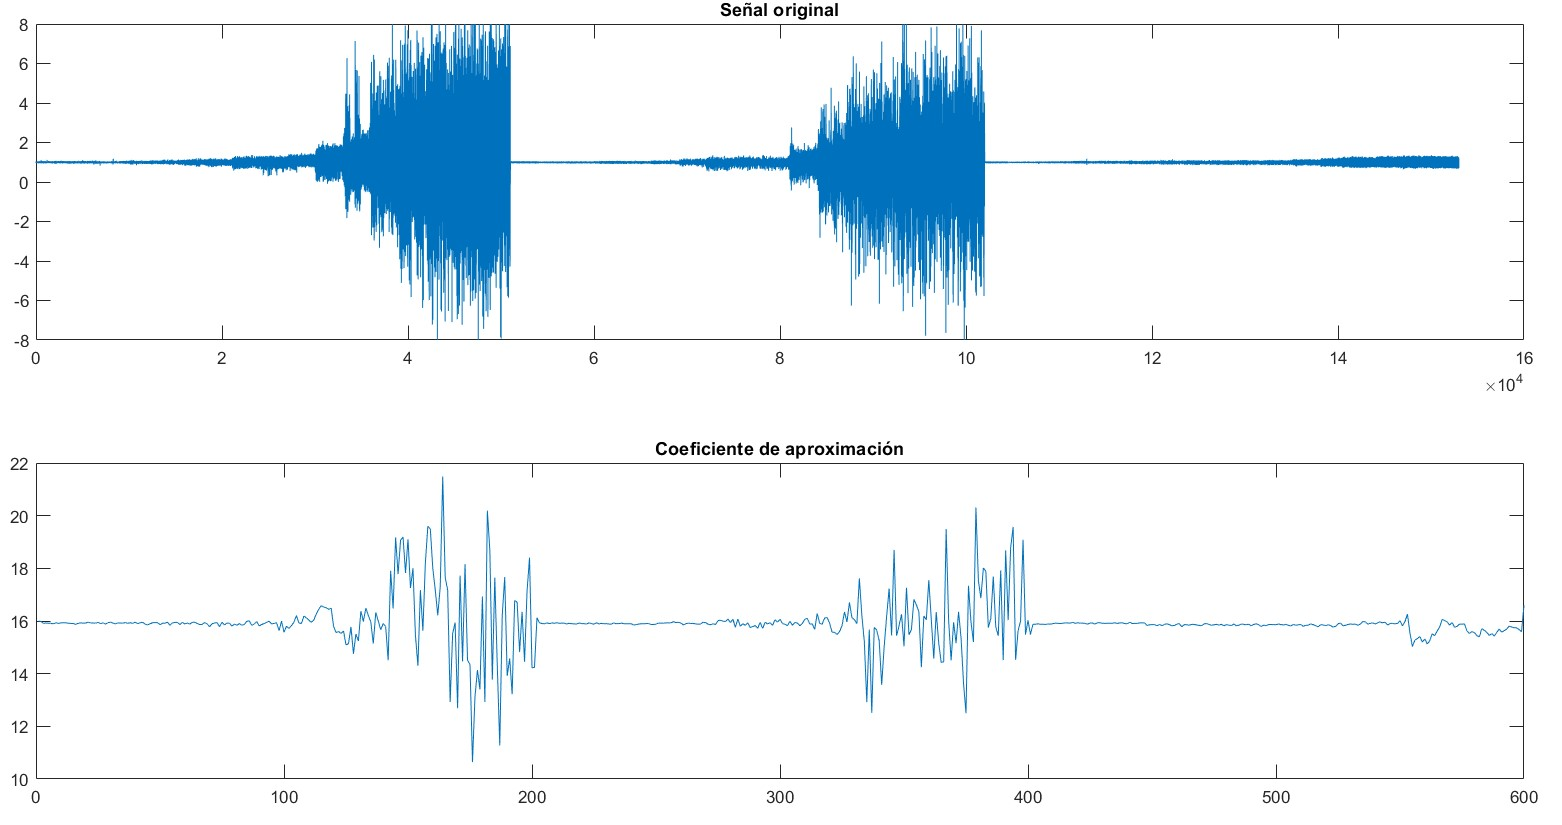
\includegraphics[scale=0.45]{original_y_wavelet_x}
	\caption{Señal original y su transformada Wavelet}
\end{figure}

\section{Conclusiones}
Conclusiones al fin xd

\bibliographystyle{ieeetr}
\begin{thebibliography}{x}
	\bibitem{accel_cite} \textsc{Scalabrini Sampaio,Gustavo, Rabello de Aguiar Vallim Filho,Arnaldo, Santos de Silva,Leilton, and Augusto da Silva,Leandro}. (2023). \textit{Accelerometer}. UCI Machine Learning Repository. \url{https://doi.org/10.24432/C5Q61V}.
	
	\bibitem{fourier} \textsc{Nussbaumer, Henri J., and Henri J. Nussbaumer.} \textit{The fast Fourier transform.} Springer Berlin Heidelberg, 1982.
	
	\bibitem{intar} \textit{Transformada Wavelet - acervo para el mejoramiento del aprendizaje de alumnos de ingeniería, en Inteligencia Artificial}.(s.f). \url{https://virtual.cuautitlan.unam.mx/intar/?page\_id=1108}
	
	\bibitem{analisis_vibr} \textsc{SAAVEDRA, Pedro Nelson}. \textit{La medición y análisis de las vibraciones como técnica de inspección de equipos y componentes, aplicaciones, normativas y certificación}. Fac. Ing.-Univ. Concepc. Chile, 2011.
	
	\bibitem{signal_processing} \textsc{MEDINA, Julio}. \textit{Análisis de Fourier para el tratamiento de señales}. Proc. XII Encuentro de Matemáticas y sus Aplicaciones, EPN-Quito, Ecuador, 2010.
	
\end{thebibliography}

\end{document}